
%(BEGIN_QUESTION)
% Copyright 2009, Tony R. Kuphaldt, released under the Creative Commons Attribution License (v 1.0)
% This means you may do almost anything with this work of mine, so long as you give me proper credit

Undersok denne P\&ID for et kaskadert gass-trykkreguleringssystem:

$$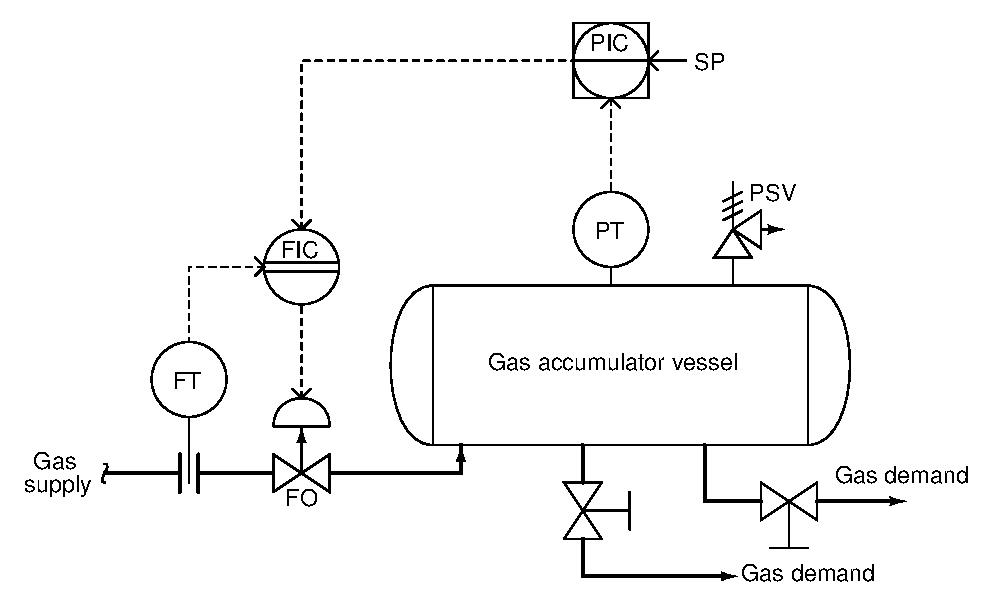
\includegraphics[width=15.5cm]{i00079x01.eps}$$

Forutsatt at begge transmittere er direkte-indikerende (dvs. hoyere trykk/strom gir hoyere signal til de respektive regulatorene), bestem nodvendig regulatorvirkning (direkte eller revers) for hver regulator.  I tillegg til a bestemme ``direkte'' eller ``revers'' virkning for hver regulator, merk hver regulators innganger med ``+'' og ``$-$'' symboler som viser virkningsretning for PV og for SP hver for seg.

\vskip 10pt

\begin{itemize}
\item{} Trykkindikerende regulator (PIC): {\it direkte} eller {\it revers} virkning?
\vskip 10pt 
\item{} Stromindikerende regulator (FIC): {\it direkte} eller {\it revers} virkning?
\end{itemize}

\vskip 20pt \vbox{\hrule \hbox{\strut \vrule{} {\bf Forslag til sokratisk diskusjon} \vrule} \hrule}

\begin{itemize}
\item{} Hva ma konfigureres i FIC for a la operatoren se 0-100\% (registrert pa regulatorens front) som sann ventilposisjon (dvs. 0\% pa front = lukket ventil og 100\% pa front = apen ventil)?
\item{} Ville svarene dine vaere annerledes hvis reguleringsventilen strupet gass som {\it forlater} karet i stedet for gass som {\it gar inn} i karet?  Dette ville selvsagt bety at minst ett av de (na) utgaende rorene ma levere gass til karet i stedet.
\item{} Ville svarene dine vaere annerledes hvis reguleringsventilen var fail-closed (FC) i stedet for fail-open (FO)?
\item{} Ville svarene dine vaere annerledes hvis stromtransmitteren var plassert nedstroms reguleringsventilen i stedet for oppstroms?
\item{} Beskriv formålet med enheten merket ``PSV'' i dette diagrammet.
\end{itemize}

\underbar{file i00079}
%(END_QUESTION)





%(BEGIN_ANSWER)

For a hjelpe analysen av systemet (spesielt ved a merke hver regulators innganger med ``+'' og ``$-$'' symboler), er du fri til a annotere regulatorvirkningene i denne modifiserte versjonen av P\&ID-en, der hver regulator er tegnet som en operasjonsforsterker:

$$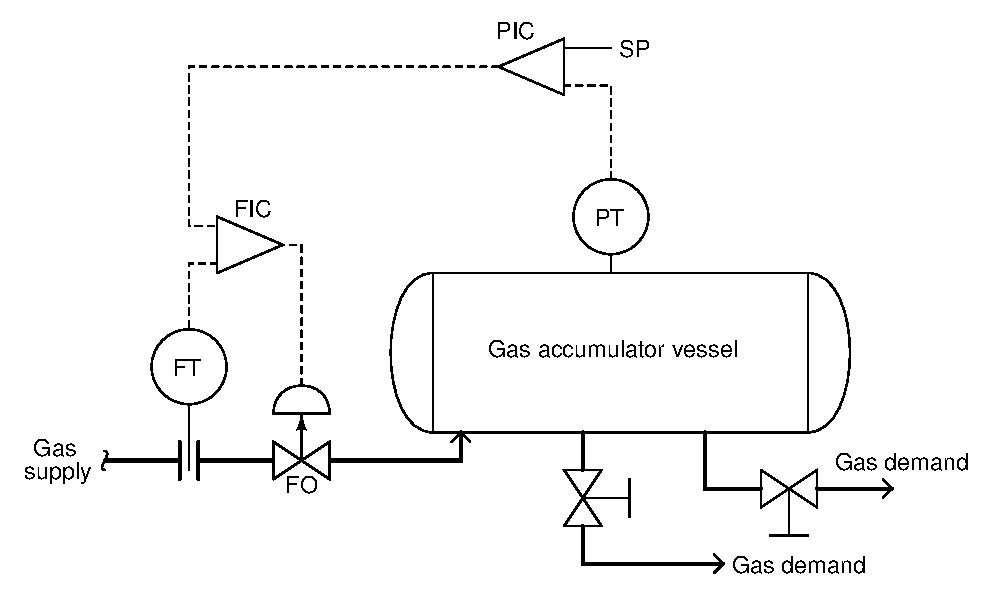
\includegraphics[width=15.5cm]{i00079x02.eps}$$

%(END_ANSWER)





%(BEGIN_NOTES)

$$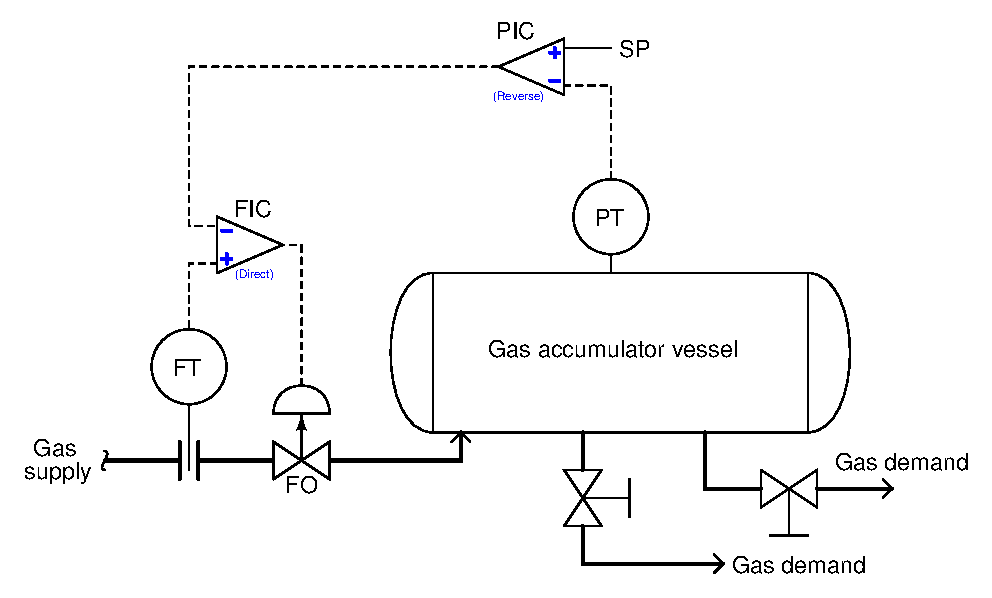
\includegraphics[width=15.5cm]{i00079x03.eps}$$







\filbreak \vskip 20pt \vbox{\hrule \hbox{\strut \vrule{} {\bf Virtuell feilsoking} \vrule} \hrule}

\noindent
{\bf Predikere effekten av en gitt feil:} presenter hver av folgende feil til studentene, en om gangen, og la dem kommentere alle effekter hver feil vil gi.

\begin{itemize}
\item{} 
\item{} 
\item{} 
\end{itemize}


\vskip 10pt


\noindent
{\bf Identifisere mulige/umulige feil:} presenter symptomer til studentene og la dem deretter avgjore om en serie foreslatte feil kan forklare alle symptomene, og forklare {\it hvorfor} eller {\it hvorfor ikke} for hver foreslatt feil:

\begin{itemize}
\item{} Symptom: {\it }
\item{}  -- {\bf Ja/Nei}
\item{}  -- {\bf Ja/Nei}
\item{}  -- {\bf Ja/Nei}
\end{itemize}


\vskip 10pt


\noindent
{\bf Vurdere nytte av gitte diagnostiske tester:} presenter symptomer til studentene og foresla deretter folgende diagnostiske tester en etter en.  Studentene vurderer verdien av hver test og avgjor om den vil gi nyttig informasjon (dvs. fortelle oss noe vi ikke allerede vet).  Studentene avgjor hva ulike resultater for hver test eventuelt indikerer om feilen, hvis noe:

\begin{itemize}
\item{} Symptom: {\it Trykket i gassakkumulator-karet oscillerer rundt setpunkt}
\item{} Sett PIC i manuell modus -- {\bf Ja}
\item{} Sjekk kalibrering av PT -- {\bf Nei}
\item{} Sjekk kalibrering av FT -- {\bf Nei}
\item{} Sett FIC i manuell modus -- {\bf Ja}
\item{} Undersok faseskift mellom PV og SP for PIC -- {\bf Nei}
\item{} Undersok faseskift mellom PV og utgang for PIC -- {\bf Ja}
\item{} Reduser gain pa PIC -- {\bf Ja}
\item{} Overvak gassettersporselsstrommer (hvis FT-er finnes nedstroms) -- {\bf Ja}
\end{itemize}


\vskip 10pt


\noindent
{\bf Diagnostisere en feil basert pa gitte symptomer:} forestill deg at ??? feiler ??? i dette systemet (ikke avslor feilen til studentene!).  Presenter operatørens observasjon(er) til studentene, la dem vurdere mulige feil og diagnostiske strategier, og gi dem deretter resultatene av tester de foreslar basert pa folgende symptomer, til de korrekt har identifisert feilens art og plassering:

\begin{itemize}
\item{} Operatørobservasjon: {\it }
\item{} 
\item{} 
\end{itemize}













\vfil \eject

\noindent
{\bf Oppsummeringsquiz:}

Identifiser effekten av at stromtransmitteren feiler med et {\it hoyt} signal (dvs. rapporterer full strom hele tiden) pa dette kaskaderte gass-trykkreguleringssystemet:

$$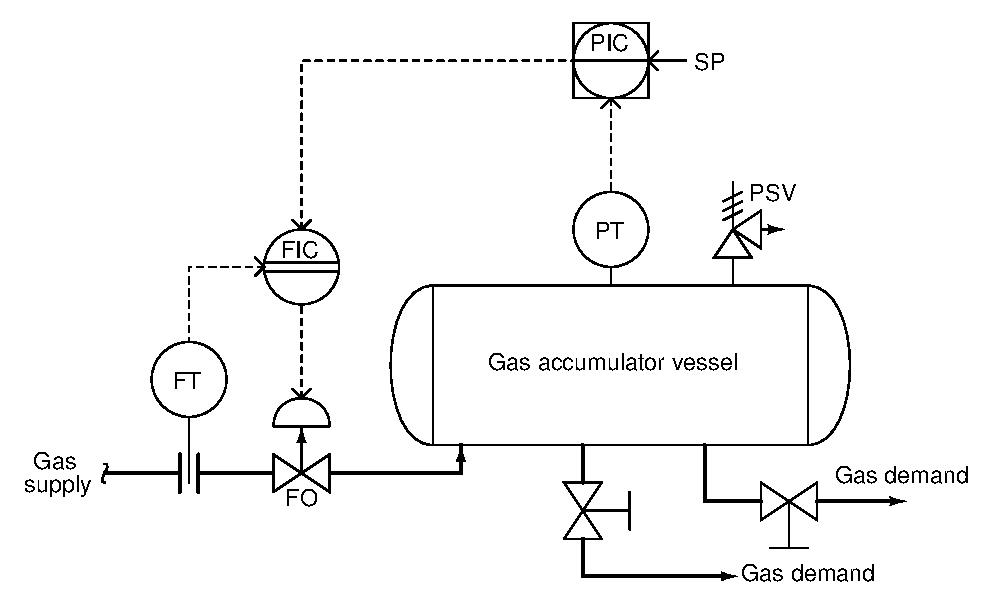
\includegraphics[width=15.5cm]{i00079x01.eps}$$

\begin{itemize}
\item{} Reguleringsventilen vil feile helt apen
\vskip 5pt 
\item{} Akkumulatorens gasstrykk vil falle under setpunkt
\vskip 5pt 
\item{} Strom gjennom ``Gas Demand''-linjene vil okes kraftig
\vskip 5pt 
\item{} Akkumulatorens gasstrykk vil stige over setpunkt 
\vskip 5pt 
\item{} Stromregulatoren vil begynne a ``sykle'' (oscillere)
\vskip 5pt 
\item{} Det vil ikke vaere noen effekt(er) overhodet pa reguleringssystemet
\end{itemize}

%INDEX% Control, strategies: cascaded controller action
%INDEX% Process: fuel gas receiver pressure control

%(END_NOTES)

